\documentclass[10pt,aspectratio=43,mathserif,table]{beamer} 
%设置为 Beamer 文档类型,设置字体为 10pt,长宽比为4:3,数学字体为 serif 风格
\batchmode

\usepackage{graphicx}
\usepackage{animate}
\usepackage{hyperref}

%导入一些用到的宏包
\usepackage{amsmath,bm,amsfonts,amssymb,enumerate,epsfig,bbm,calc,color,ifthen,capt-of,multimedia,hyperref}
\usepackage{ctex} %导入中文包
\setCJKmainfont{SimHei} %字体可采用黑体  Microsoft YaHei
% \setCJKmainfont{FandolKai} %Overleaf中字体只能这条,采用楷体等见overleaf字体说明

\usetheme{Berlin} %主题
\usecolortheme{sustech} %主题颜色

\usepackage[ruled,linesnumbered]{algorithm2e}

\usepackage{fancybox}
\usepackage{xcolor}
\usepackage{times}
\usepackage{listings}

\usepackage{booktabs}
\usepackage{colortbl}
\usepackage{multicol}

\usepackage{tikz}
\usetikzlibrary{calc}
\usetikzlibrary{intersections,through}
\usetikzlibrary{decorations.pathreplacing}

\setsansfont{Microsoft YaHei} %设置非衬线字体采用黑体  Microsoft YaHei
% \setsansfont{SimHei} %可设置非衬线字体
\setmainfont{Times New Roman} %设置英文字体采用 Times New Roman,overleaf中有效,其他可能需要将上方非衬线字体设置删除

\definecolor{mygreen}{rgb}{0,0.6,0}
\definecolor{mymauve}{rgb}{0.58,0,0.82}
\definecolor{mygray}{gray}{.9}
\definecolor{mypink}{rgb}{.99,.91,.95}
\definecolor{mycyan}{cmyk}{.3,0,0,0}

%题目,作者,学校,日期
\title{演示报告 \quad(内容为示例简述特征向量)}
\subtitle{\fontsize{9pt}{14pt}\textbf{标题小字 \quad(示例全英,可自行修改为中文)}}
\author{Yi Wang(姓名)  \newline \newline \fontsize{6pt}{10pt}数学与统计学院}
\institute{\fontsize{6pt}{10pt}广东工业大学 \newline Guangdong University of Tech.}
\date{\today}

% 学校Logo
\logo{
\includegraphics[height=1cm]{./fig/logo.png}\hspace*{0.1cm}}

\AtBeginSection[]
{
	\begin{frame}<beamer>
	\frametitle{\textbf{CONTENT}}
	\tableofcontents[currentsection]
\end{frame}
}
\beamerdefaultoverlayspecification{<+->}
% -----------------------------------------------------------------------------
\begin{document}
% -----------------------------------------------------------------------------

\frame{\titlepage}

\section[CONTENT]{}   %目录
\begin{frame}{CONTENT}
	\tableofcontents
\end{frame}

% -----------------------------------------------------------------------------
\section{图片与枚举示例}  %引言

\begin{frame}{Review of Higher Algebra}
	\begin{multicols}{2}
		
\includegraphics[height=4cm]{fig/gaodai_cover.jpg}
		\begin{itemize}
			\item Full of matrix
			\item No geometric graphics at all
			\item Not intuitive
		\end{itemize}
	\end{multicols}
\end{frame}
\begin{frame}{Review of Higher Algebra}
	\begin{multicols}{2}
		
\includegraphics[height=4cm]{fig/gaodai.jpg}
		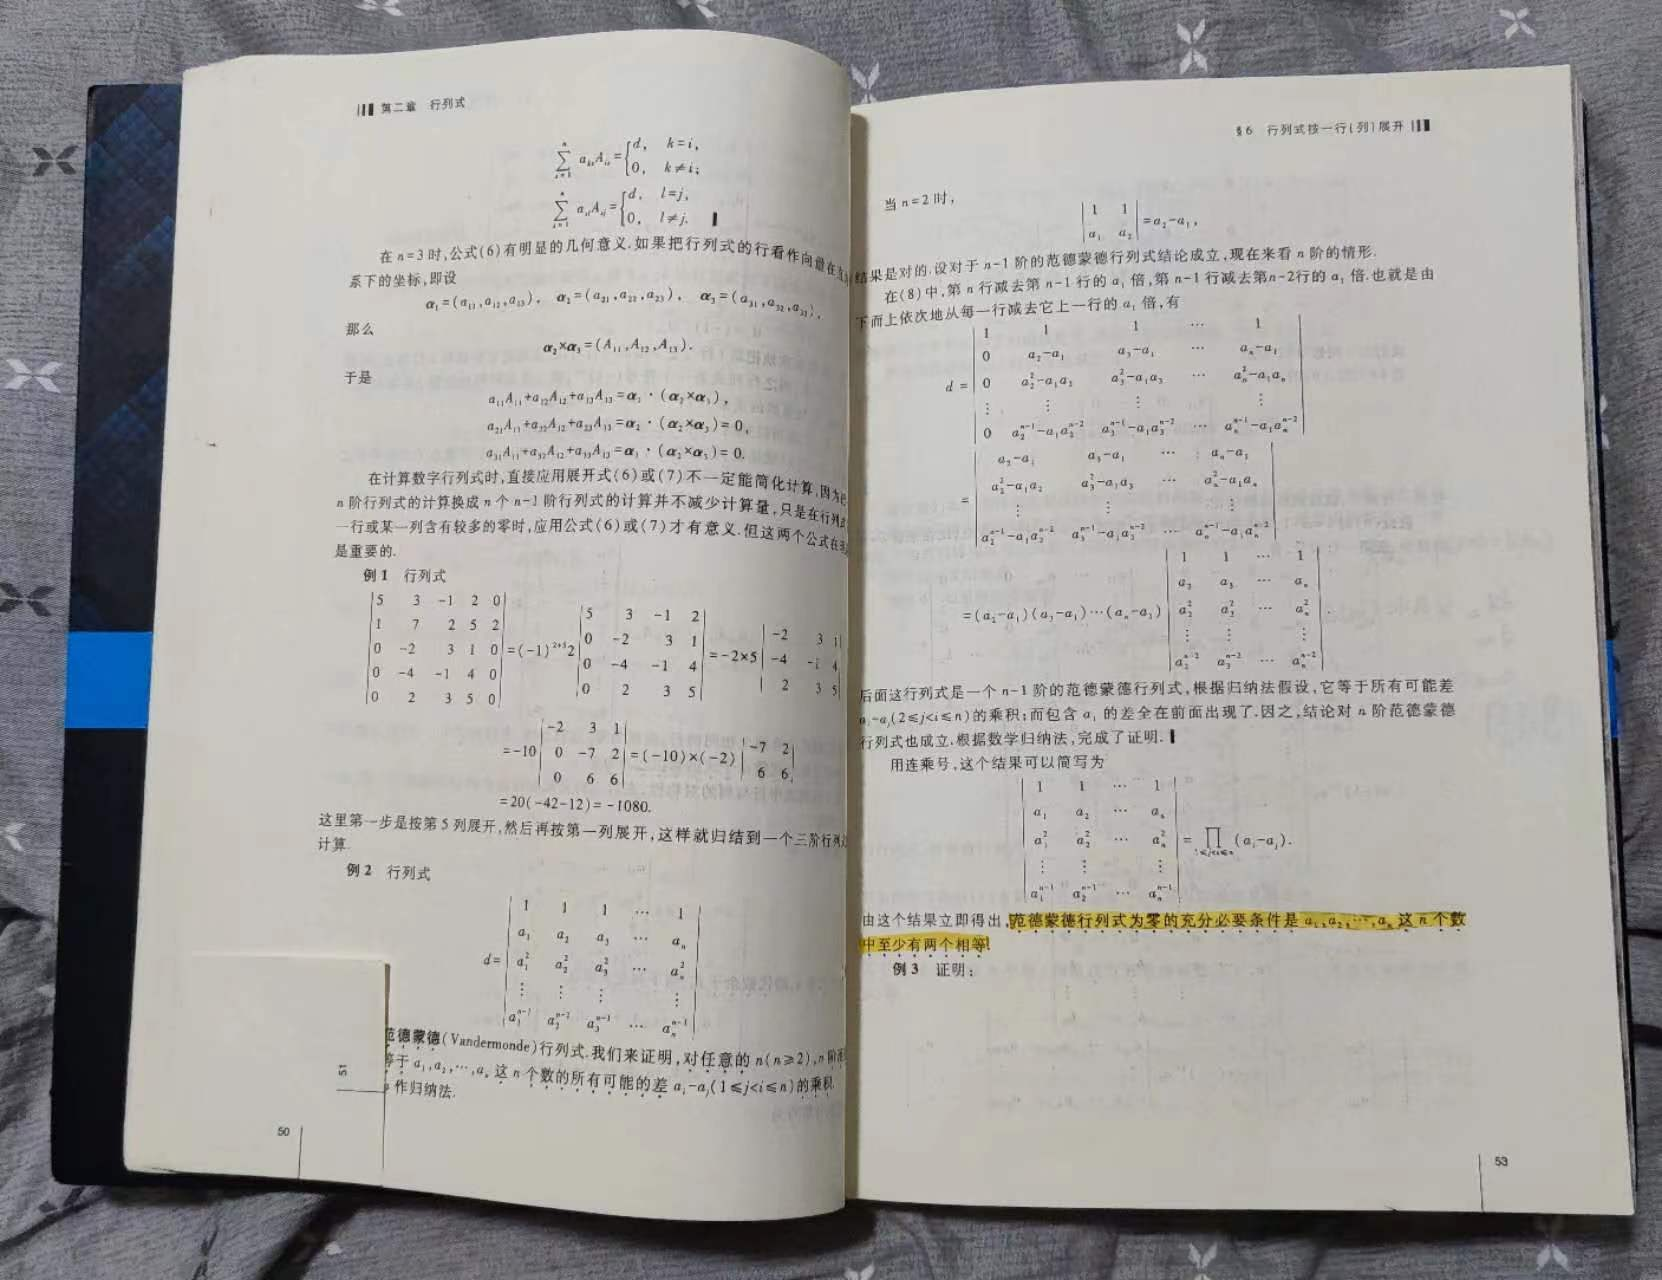
\includegraphics[height=4cm]{fig/gaodai_mat.jpg}
	\end{multicols}
\end{frame}


\section{公式显示示例 Vector in Geometry}
\begin{frame}{Linear Simultaneous Equations}
	Introduce a linear simultaneous equations
	\begin{equation}
		\begin{aligned}
			 & x  & - & \quad 2y & = 1  \\
			 & 3x & + & \quad 2y & = 11
		\end{aligned}
	\end{equation}
	\begin{multicols}{2} % 分两栏 若花括号中为3则是分三列
		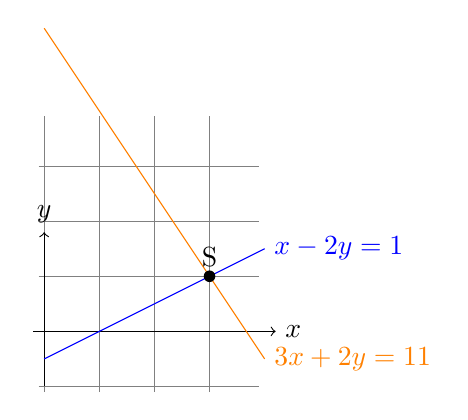
\begin{tikzpicture}[scale=0.7,domain=0:4]
			\draw[very thin,color=gray] (-0.1,-1.1) grid (3.9,3.9);
			\draw[->] (-0.2,0) -- (4.2,0) node[right] {$x$};
			\draw[->] (0,-1) -- (0,1.8) node[above] {$y$};
			\draw[color=blue] plot (\x,{\x/2 -0.5)}) node[right] {$x - 2y =1$};
			\draw[color=orange] plot (\x,{-1.5*\x +5.5)}) node[right] {$3x+2y=11$};
			\coordinate [label=S] (O) at (3,1);
			\fill (O) circle(3pt);
		\end{tikzpicture}
		\hfill
		\quad\\[0.5cm]
		Row picture:\\[0.1cm]
		\fbox{x - 2y =1}\\
		\fbox{3x+2y=11}\\[0.1cm]
		Point $S=(3,1)$ is the solution.
	\end{multicols}
\end{frame}

\begin{frame}{Vector}
	Column picture:\\
	\begin{equation}
		x\left[\begin{array}{c}
				1 \\
				3 \\
			\end{array}\right]
		+y\left[\begin{array}{r}
				-2 \\
				2  \\
			\end{array}\right]
		=\left[\begin{array}{r}
				1  \\
				11 \\
			\end{array}\right]
	\end{equation}
	\begin{multicols}{3} % 分两栏 若花括号中为3则是分三列
		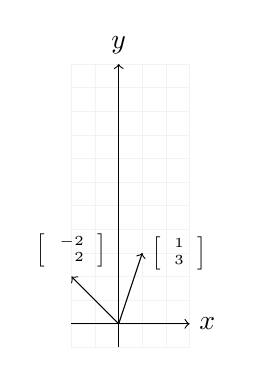
\begin{tikzpicture}[scale=0.3,domain=-2:2]
			\draw[very thin,color=gray,opacity=0.1] (-2,-1) grid (3,11);
			\draw[->] (-2,0) -- (3,0) node[right] {$x$};
			\draw[->] (0,-1) -- (0,11) node[above] {$y$};
			\draw[->] (0,0) -- (-2,2) node[above] {\tiny{$\left[\begin{array}{r}
								-2 \\
								2  \\
							\end{array}\right]$}};
			\draw[->] (0,0) -- (1,3) node[right] {\tiny{$\left[\begin{array}{c}
								1 \\
								3 \\
							\end{array}\right]$}};
		\end{tikzpicture}
		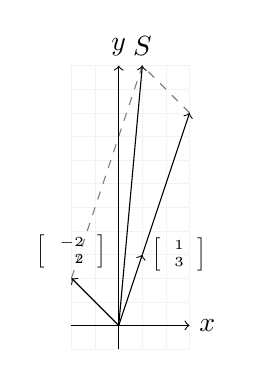
\begin{tikzpicture}[scale=0.3,domain=-2:2]
			\draw[very thin,color=gray,opacity=0.1] (-2,-1) grid (3,11);
			\draw[->] (-2,0) -- (3,0) node[right] {$x$};
			\draw[->] (0,-1) -- (0,11) node[above] {$y$};
			\draw[->] (0,0) -- (-2,2) node[above] {\tiny{$\left[\begin{array}{r}
								-2 \\
								2  \\
							\end{array}\right]$}};
			\draw[->] (0,0) -- (1,3) node[right] {\tiny{$\left[\begin{array}{c}
								1 \\
								3 \\
							\end{array}\right]$}};
			\draw[->] (1,3) -- (3,9) node[above]{} ;
			\draw[dashed,opacity=0.5] (-2,2) -- (1,11);
			\draw[dashed,opacity=0.5] (3,9) -- (1,11);
			\draw[->] (0,0) -- (1,11) node[above]{$S$} ;
		\end{tikzpicture}
		\hfill
		Where we take
		\\[0.2cm]
		$\left[\begin{array}{r}
					-2 \\
					2  \\
				\end{array}\right]$ and $\left[\begin{array}{c}
					1 \\
					3 \\
				\end{array}\right]$ \\[0.2cm]
		as vectors,\\[0.2cm]
		when $x=3$,\quad $y=1$ ,the $b = \left[\begin{array}{r}
					1  \\
					11 \\
				\end{array}\right]$
	\end{multicols}
\end{frame}

\section{公式显示示例 Determinant in Geometry}
\begin{frame}{Coefficient matrix}
	$$	\left[\begin{array}{rr}
				3 & 1 \\
				0 & 2 \\
			\end{array}\right]
		\left[\begin{array}{r}
				x \\
				y \\
			\end{array}\right]
		=\left[\begin{array}{r}
				\cdots \\
				\cdots \\
			\end{array}\right]
		or
		\left[\begin{array}{rr}
				3 & 1 \\
				0 & 2 \\
			\end{array}\right]
		\left[\begin{array}{r}
				a \\
				b \\
			\end{array}\right]
		=\left[\begin{array}{r}
				\cdots \\
				\cdots \\
			\end{array}\right]
	$$
	Coefficient matrix
	$	A = 	\left[\begin{array}{rr}
				3 & 1 \\
				0 & 2 \\
			\end{array}\right]
	$
	is also a rectangular matrix.\\[0.2cm]
	$det(A) = \left|\begin{array}{rr}
			3 & 1 \\
			0 & 2 \\
		\end{array}\right| =6$\\[0.2cm]
	Obvious matrix A has two vectors:$		\left[\begin{array}{r}
				3 \\
				0 \\
			\end{array}\right]
	$,
	$		\left[\begin{array}{r}
				1 \\
				2 \\
			\end{array}\right]
	$
\end{frame}

\begin{frame}{公式显示示例 Linear transformations}
	Unit vectors in the 2-dimensional plane are $\hat{i}=\left[\begin{array}{r}
				1 \\
				0 \\
			\end{array}\right]$ , $\hat{j}=\left[\begin{array}{r}
				0 \\
				1 \\
			\end{array}\right]$.\\[0.5cm]
	\begin{multicols}{3}
		$a\cdot i + b\cdot j $\\[0.1cm]
		$=a\left[\begin{array}{r}
					1 \\
					0 \\
				\end{array}\right]
			+b\left[\begin{array}{r}
					0 \\
					1 \\
				\end{array}\right]$\\[0.1cm]
		$=\left[\begin{array}{r}
					a \\
					b \\
				\end{array}\right]$\quad
		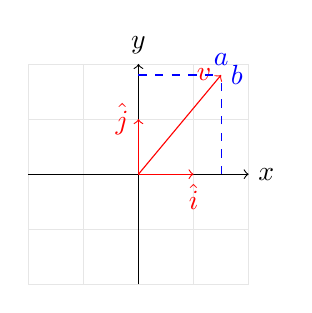
\begin{tikzpicture}[scale=0.7,domain=-2:2]
			\draw[very thin,color=gray,opacity=0.2] (-2,-2) grid (2,2);
			\draw[->] (-2,0) -- (2,0) node[right] {$x$};
			\draw[->] (0,-2) -- (0,2) node[above] {$y$};
			\draw[->,color=red] (0,0)--(1,0) node[below]{$\hat{i}$};
			\draw[->,color=red] (0,0)--(0,1) node[left]{$\hat{j}$};
			\draw[->,color=red] (0,0)--(1.5,1.8) node[left]{$v$};
			\draw[dashed,color=blue] (1.5,0)--(1.5,1.8) node[right]{$b$};
			\draw[dashed,color=blue] (0,1.8)--(1.5,1.8) node[above]{$a$};
		\end{tikzpicture}\\[0.2cm]
		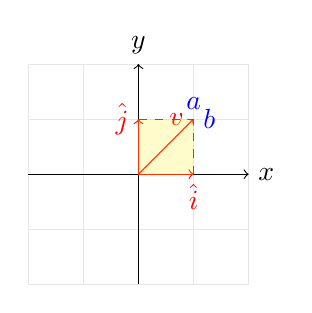
\begin{tikzpicture}[scale=0.7,domain=-2:2]
			\draw[very thin,color=gray,opacity=0.2] (-2,-2) grid (2,2);
			\draw[->] (-2,0) -- (2,0) node[right] {$x$};
			\draw[->] (0,-2) -- (0,2) node[above] {$y$};
			\draw[->,color=red] (0,0)--(1,0) node[below]{$\hat{i}$};
			\draw[->,color=red] (0,0)--(0,1) node[left]{$\hat{j}$};
			\draw[->,color=red] (0,0)--(1,1) node[left]{$v$};
			\draw[dashed,color=blue] (1,0)--(1,1) node[right]{$b$};
			\draw[dashed,color=blue] (0,1)--(1,1) node[above]{$a$};
			\filldraw[color=yellow,opacity=0.2] (0,0) -- (1,0) -- (1,1) -- (0,1);
		\end{tikzpicture}\\[0.2cm]

	\end{multicols}


	\fbox{$a\cdot i + b\cdot j $} is a linear transformations.\quad $a=1,b=1 $,then area is $1 $.\\[0.2cm]
	also $\left[\begin{array}{rr}
				i & j \\
			\end{array}\right]\left[\begin{array}{r}
				a \\
				b \\
			\end{array}\right] = \left[\begin{array}{r}
				a \\
				b \\
			\end{array}\right]$\quad $\Rightarrow$ \quad
	$\left[\begin{array}{rr}
				1 & 0 \\
				0 & 1 \\
			\end{array}\right]\left[\begin{array}{r}
				a \\
				b \\
			\end{array}\right] = \left[\begin{array}{r}
				a \\
				b \\
			\end{array}\right]$
\end{frame}

\begin{frame}
	Hense, we can tell that	\\[0.2cm]
	$	\left[\begin{array}{rr}
				3 & 1 \\
				0 & 2 \\
			\end{array}\right]
		\left[\begin{array}{r}
				a \\
				b \\
			\end{array}\right]
	$
	$
		= \left[\begin{array}{rr}
				3 & 1 \\
				0 & 2 \\
			\end{array}\right]
		\left[\begin{array}{rr}
				1 & 0 \\
				0 & 1 \\
			\end{array}\right]
		\left[\begin{array}{r}
				a \\
				b \\
			\end{array}\right]
	$\\[0.2cm]
	Which is actually the original two-dimensional space of the unit vector is linearly transformed. $\rightarrow \times \left[\begin{array}{rr}
				3 & 1 \\
				0 & 2 \\
			\end{array}\right]$\\[0.2cm]
	$\hat{i} = \left[\begin{array}{r}
				1 \\
				0 \\
			\end{array}\right]
		\rightarrow \left[\begin{array}{r}
				3 \\
				0 \\
			\end{array}\right]
	$\quad ,\quad
	$\hat{j} = \left[\begin{array}{r}
				0 \\
				1 \\
			\end{array}\right]\rightarrow \left[\begin{array}{r}
				1 \\
				2 \\
			\end{array}\right]
	$\\[0.5cm]
	\begin{multicols}{3}
		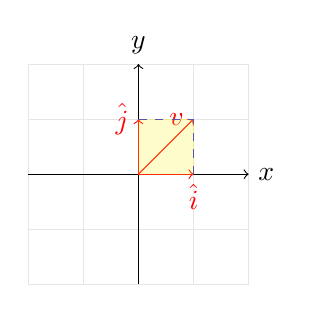
\begin{tikzpicture}[scale=0.7,domain=-2:2]
			\draw[very thin,color=gray,opacity=0.2] (-2,-2) grid (2,2);
			\draw[->] (-2,0) -- (2,0) node[right] {$x$};
			\draw[->] (0,-2) -- (0,2) node[above] {$y$};
			\draw[->,color=red] (0,0)--(1,0) node[below]{$\hat{i}$};
			\draw[->,color=red] (0,0)--(0,1) node[left]{$\hat{j}$};
			\draw[->,color=red] (0,0)--(1,1) node[left]{$v$};
			\draw[dashed,color=blue] (1,0)--(1,1) node[right]{};
			\draw[dashed,color=blue] (0,1)--(1,1) node[above]{};
			\filldraw[color=yellow,opacity=0.2] (0,0) -- (1,0) -- (1,1) -- (0,1);
		\end{tikzpicture}\\[1cm]
		\hfill

		$$\Rightarrow$$
		Area : $1 \rightarrow 6$\\[0.1cm]
		\hfill
		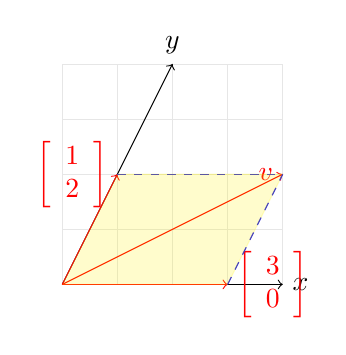
\begin{tikzpicture}[scale=0.7,domain=-2:2]
			\draw[very thin,color=gray,opacity=0.2] (0,0) grid (4,4);
			\draw[->] (0,0) -- (4,0) node[right] {$x$};
			\draw[->] (0,0) -- (2,4) node[above] {$y$};
			\draw[->,color=red] (0,0)--(3,0) node[right]{$\left[\begin{array}{r}
							3 \\
							0 \\
						\end{array}\right]$};
			\draw[->,color=red] (0,0)--(1,2) node[left]{$\left[\begin{array}{r}
							1 \\
							2 \\
						\end{array}\right]$};
			\draw[->,color=red] (0,0)--(4,2) node[left]{$v$};
			\draw[dashed,color=blue] (3,0)--(4,2) node[right]{};
			\draw[dashed,color=blue] (1,2)--(4,2) node[above]{};
			\filldraw[color=yellow,opacity=0.2] (0,0) -- (3,0) -- (4,2) -- (1,2);
		\end{tikzpicture}
	\end{multicols}

\end{frame}



\begin{frame}{Determinant in Geometry}
	Since
	$\left|\begin{array}{rr}
			3 & 1 \\
			0 & 2 \\
		\end{array}\right|
		= 6
	$ ,\quad
	Area : $1 \rightarrow 6$\\[0.2cm]
	\begin{multicols}{3}
		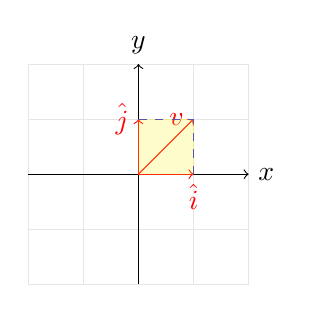
\begin{tikzpicture}[scale=0.7,domain=-2:2]
			\draw[very thin,color=gray,opacity=0.2] (-2,-2) grid (2,2);
			\draw[->] (-2,0) -- (2,0) node[right] {$x$};
			\draw[->] (0,-2) -- (0,2) node[above] {$y$};
			\draw[->,color=red] (0,0)--(1,0) node[below]{$\hat{i}$};
			\draw[->,color=red] (0,0)--(0,1) node[left]{$\hat{j}$};
			\draw[->,color=red] (0,0)--(1,1) node[left]{$v$};
			\draw[dashed,color=blue] (1,0)--(1,1) node[right]{};
			\draw[dashed,color=blue] (0,1)--(1,1) node[above]{};
			\filldraw[color=yellow,opacity=0.2] (0,0) -- (1,0) -- (1,1) -- (0,1);
		\end{tikzpicture}\\[1cm]
		\hfill

		$$\Rightarrow$$
		Area scaled \\[0.1cm]
		by \textbf{6} times.\\[0.1cm]
		\hfill
		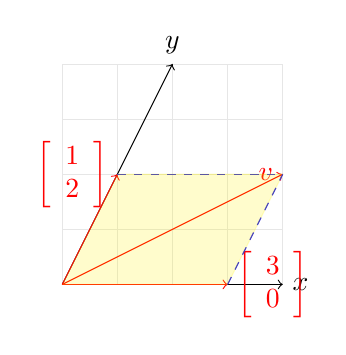
\begin{tikzpicture}[scale=0.7,domain=-2:2]
			\draw[very thin,color=gray,opacity=0.2] (0,0) grid (4,4);
			\draw[->] (0,0) -- (4,0) node[right] {$x$};
			\draw[->] (0,0) -- (2,4) node[above] {$y$};
			\draw[->,color=red] (0,0)--(3,0) node[right]{$\left[\begin{array}{r}
							3 \\
							0 \\
						\end{array}\right]$};
			\draw[->,color=red] (0,0)--(1,2) node[left]{$\left[\begin{array}{r}
							1 \\
							2 \\
						\end{array}\right]$};
			\draw[->,color=red] (0,0)--(4,2) node[left]{$v$};
			\draw[dashed,color=blue] (3,0)--(4,2) node[right]{};
			\draw[dashed,color=blue] (1,2)--(4,2) node[above]{};
			\filldraw[color=yellow,opacity=0.2] (0,0) -- (3,0) -- (4,2) -- (1,2);
		\end{tikzpicture}
	\end{multicols}


	We can conclude that :\\[0.2cm]
	The Determinant in Geometry
	is how much are areas scaled.
\end{frame}


\section{公式显示示例 Eigenvalue in Geometry}
\begin{frame}{Vectors remain on their own span}
	\hspace{-2cm}{
		\begin{multicols}{3}
			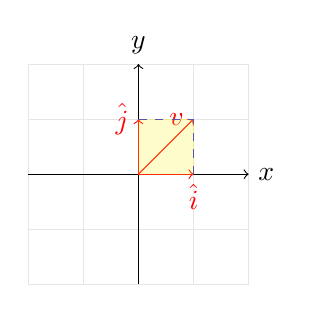
\begin{tikzpicture}[scale=0.7,domain=-2:2]
				\draw[very thin,color=gray,opacity=0.2] (-2,-2) grid (2,2);
				\draw[->] (-2,0) -- (2,0) node[right] {$x$};
				\draw[->] (0,-2) -- (0,2) node[above] {$y$};
				\draw[->,color=red] (0,0)--(1,0) node[below]{$\hat{i}$};
				\draw[->,color=red] (0,0)--(0,1) node[left]{$\hat{j}$};
				\draw[->,color=red] (0,0)--(1,1) node[left]{$v$};
				\draw[dashed,color=blue] (1,0)--(1,1) node[right]{};
				\draw[dashed,color=blue] (0,1)--(1,1) node[above]{};
				\filldraw[color=yellow,opacity=0.2] (0,0) -- (1,0) -- (1,1) -- (0,1);
			\end{tikzpicture}\\[1cm]
			\hfill

			linearly transformed.\\[0.2cm]
			$\rightarrow \times \left[\begin{array}{rr}
						3 & 1 \\
						0 & 2 \\
					\end{array}\right]
				\rightarrow$\\[0.2cm]
			\hfill
			\hspace{-1.8cm}
			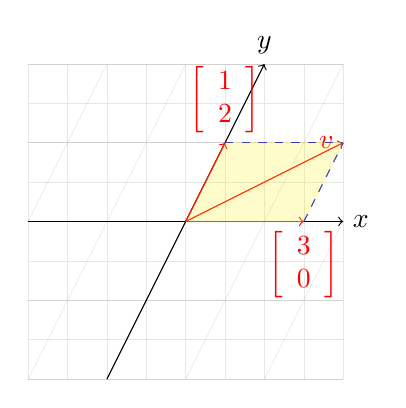
\begin{tikzpicture}[scale=0.5,domain=-2:2]
				\draw[very thin,color=gray,opacity=0.2] (-4,-4) grid (4,4);
				\draw[very thin,color=gray,opacity=0.2] (-4,0) -- (4,0) ;
				\draw[very thin,color=gray,opacity=0.2] (-4,2) -- (4,2) ;
				\draw[very thin,color=gray,opacity=0.2] (-4,4) -- (4,4) ;
				\draw[very thin,color=gray,opacity=0.2] (-4,-2) -- (4,-2) ;
				\draw[very thin,color=gray,opacity=0.2] (-4,-4) -- (4,-4) ;

				\draw[very thin,color=gray,opacity=0.2] (-4,-0) -- (-2,4) ;
				\draw[very thin,color=gray,opacity=0.2] (-4,-4) -- (0,4) ;
				\draw[very thin,color=gray,opacity=0.2] (-2,-4) -- (2,4) ;
				\draw[very thin,color=gray,opacity=0.2] (0,-4) -- (4,4) ;
				\draw[very thin,color=gray,opacity=0.2] (2,-4) -- (4,0) ;

				\draw[->] (-4,0) -- (4,0) node[right] {$x$};
				\draw[->] (-2,-4) -- (2,4) node[above] {$y$};
				\draw[->,color=red] (0,0)--(3,0) node[below]{$\left[\begin{array}{r}
								3 \\
								0 \\
							\end{array}\right]$};
				\draw[->,color=red] (0,0)--(1,2) node[above]{$\left[\begin{array}{r}
								1 \\
								2 \\
							\end{array}\right]$};
				\draw[->,color=red] (0,0)--(4,2) node[left]{$v$};
				\draw[dashed,color=blue] (3,0)--(4,2) node[right]{};
				\draw[dashed,color=blue] (1,2)--(4,2) node[above]{};
				\filldraw[color=yellow,opacity=0.2] (0,0) -- (3,0) -- (4,2) -- (1,2);
			\end{tikzpicture}
		\end{multicols}}
\end{frame}

\begin{frame}{Vectors remain on their own span}
	\begin{multicols}{3}
		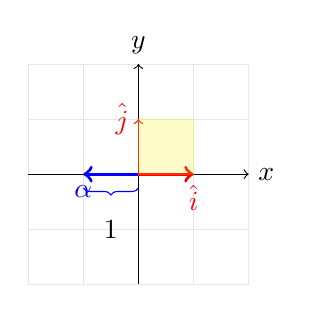
\begin{tikzpicture}[scale=0.7,domain=-2:2]
			\draw[very thin,color=gray,opacity=0.2] (-2,-2) grid (2,2);
			\draw[->] (-2,0) -- (2,0) node[right] {$x$};
			\draw[->] (0,-2) -- (0,2) node[above] {$y$};
			\draw[very thick,->,color=red] (0,0)--(1,0) node[below]{$\hat{i}$};
			\draw[very thick,->,color=blue] (0,0)--(-1,0) node[below]{$\alpha$};
			\draw[decorate,decoration={brace,raise=5pt},blue] (0,0)--(-1,0);
			\node at (-0.5,-1) {1};
			\draw[->,color=red] (0,0)--(0,1) node[left]{$\hat{j}$};
			\filldraw[color=yellow,opacity=0.2] (0,0) -- (1,0) -- (1,1) -- (0,1);
		\end{tikzpicture}\\[1cm]
		\hfill

		linearly transformed.\\[0.2cm]
		$\rightarrow \times \left[\begin{array}{rr}
					3 & 1 \\
					0 & 2 \\
				\end{array}\right]
			\rightarrow$\\[0.2cm]
		\hfill
		\hspace{-1.8cm}
		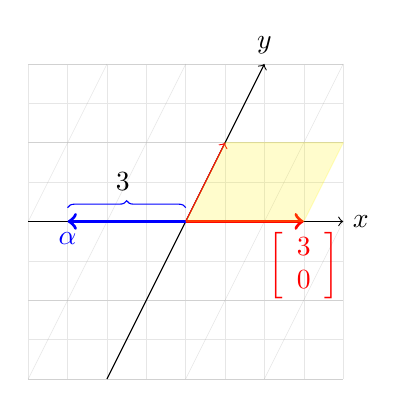
\begin{tikzpicture}[scale=0.5,domain=-2:2]
			\draw[very thin,color=gray,opacity=0.2] (-4,-4) grid (4,4);
			\draw[very thin,color=gray,opacity=0.2] (-4,0) -- (4,0) ;
			\draw[very thin,color=gray,opacity=0.2] (-4,2) -- (4,2) ;
			\draw[very thin,color=gray,opacity=0.2] (-4,4) -- (4,4) ;
			\draw[very thin,color=gray,opacity=0.2] (-4,-2) -- (4,-2) ;
			\draw[very thin,color=gray,opacity=0.2] (-4,-4) -- (4,-4) ;

			\draw[very thin,color=gray,opacity=0.2] (-4,-0) -- (-2,4) ;
			\draw[very thin,color=gray,opacity=0.2] (-4,-4) -- (0,4) ;
			\draw[very thin,color=gray,opacity=0.2] (-2,-4) -- (2,4) ;
			\draw[very thin,color=gray,opacity=0.2] (0,-4) -- (4,4) ;
			\draw[very thin,color=gray,opacity=0.2] (2,-4) -- (4,0) ;

			\draw[->] (-4,0) -- (4,0) node[right] {$x$};
			\draw[->] (-2,-4) -- (2,4) node[above] {$y$};
			\draw[very thick,->,color=red] (0,0)--(3,0) node[below]{$\left[\begin{array}{r}
							3 \\
							0 \\
						\end{array}\right]$};


			\draw[very thick,->,color=blue] (0,0)--(-3,0) node[below]{$\alpha$};
			\draw[decorate,decoration={brace,mirror,raise=5pt},blue] (0,0)--(-3,0);
			\node at (-1.6,1) {3};
			\draw[->,color=red] (0,0)--(1,2) node[above]{};

			\filldraw[color=yellow,opacity=0.2] (0,0) -- (3,0) -- (4,2) -- (1,2);
		\end{tikzpicture}
	\end{multicols}
	\textbf{$\overrightarrow{\alpha}$} remains on the line of the x-axis,stretched by a factor of \textbf{3}.
\end{frame}

\begin{frame}{Vectors remain on their own span}
	\begin{multicols}{3}
		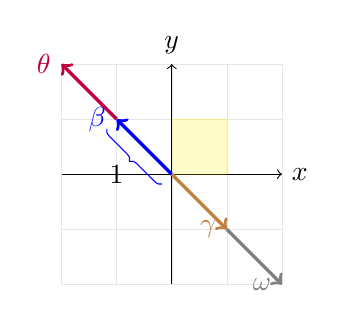
\begin{tikzpicture}[scale=0.7,domain=-2:2]
			\draw[very thin,color=gray,opacity=0.2] (-2,-2) grid (2,2);
			\draw[->] (-2,0) -- (2,0) node[right] {$x$};
			\draw[->] (0,-2) -- (0,2) node[above] {$y$};


			\draw[very thick,->,color=brown] (0,0)--(1,-1) node[left]{$\gamma$};
			\draw[very thick,->,color=purple] (-1,1)--(-2,2) node[left]{$\theta$};
			\draw[very thick,->,color=gray] (1,-1)--(2,-2) node[left]{$\omega$};

			\draw[very thick,->,color=blue] (0,0)--(-1,1) node[left]{$\beta$};
			\draw[decorate,decoration={brace,raise=5pt},blue] (0,0)--(-1,1);
			\node at (-1,0) {1};

			\filldraw[color=yellow,opacity=0.2] (0,0) -- (1,0) -- (1,1) -- (0,1);
		\end{tikzpicture}\\[1cm]
		\hfill

		linearly transformed.\\[0.2cm]
		$\rightarrow \times \left[\begin{array}{rr}
					3 & 1 \\
					0 & 2 \\
				\end{array}\right]
			\rightarrow$\\[0.2cm]
		\hfill
		\hspace{-1.8cm}
		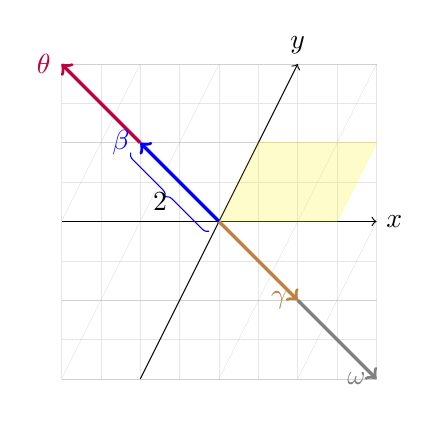
\begin{tikzpicture}[scale=0.5,domain=-2:2]
			\draw[very thin,color=gray,opacity=0.2] (-4,-4) grid (4,4);
			\draw[very thin,color=gray,opacity=0.2] (-4,0) -- (4,0) ;
			\draw[very thin,color=gray,opacity=0.2] (-4,2) -- (4,2) ;
			\draw[very thin,color=gray,opacity=0.2] (-4,4) -- (4,4) ;
			\draw[very thin,color=gray,opacity=0.2] (-4,-2) -- (4,-2) ;
			\draw[very thin,color=gray,opacity=0.2] (-4,-4) -- (4,-4) ;

			\draw[very thin,color=gray,opacity=0.2] (-4,-0) -- (-2,4) ;
			\draw[very thin,color=gray,opacity=0.2] (-4,-4) -- (0,4) ;
			\draw[very thin,color=gray,opacity=0.2] (-2,-4) -- (2,4) ;
			\draw[very thin,color=gray,opacity=0.2] (0,-4) -- (4,4) ;
			\draw[very thin,color=gray,opacity=0.2] (2,-4) -- (4,0) ;

			\draw[->] (-4,0) -- (4,0) node[right] {$x$};
			\draw[->] (-2,-4) -- (2,4) node[above] {$y$};

			\draw[very thick,->,color=brown] (0,0)--(2,-2) node[left]{$\gamma$};
			\draw[very thick,->,color=purple] (-2,2)--(-4,4) node[left]{$\theta$};
			\draw[very thick,->,color=gray] (2,-2)--(4,-4) node[left]{$\omega$};

			\draw[very thick,->,color=blue] (0,0)--(-2,2) node[left]{$\beta$};
			\draw[decorate,decoration={brace,raise=5pt},blue] (0,0)--(-2,2);
			\node at (-1.5,0.5) {2};


			\filldraw[color=yellow,opacity=0.2] (0,0) -- (3,0) -- (4,2) -- (1,2);
		\end{tikzpicture}
	\end{multicols}
	\textbf{$\overrightarrow{\beta}$} remains on the line of the x-axis,stretched by a factor of \textbf{2}.\\[0.2cm]
	The other vectors($\gamma,\theta,\omega$) on the line are also stretched by a factor of \textbf{2}
\end{frame}

\begin{frame}{Eigenvalue \& Eigenvector}
	\begin{multicols}{2}
		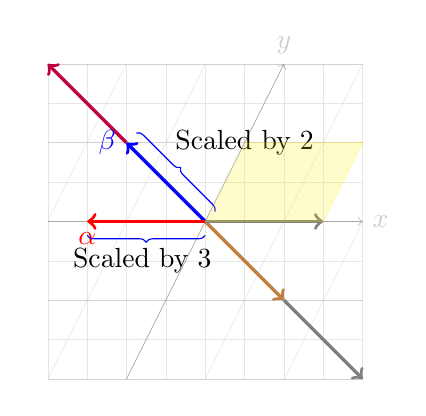
\begin{tikzpicture}[scale=0.5,domain=-2:2]
			\draw[very thin,color=gray,opacity=0.2] (-4,-4) grid (4,4);
			\draw[very thin,color=gray,opacity=0.2] (-4,0) -- (4,0) ;
			\draw[very thin,color=gray,opacity=0.2] (-4,2) -- (4,2) ;
			\draw[very thin,color=gray,opacity=0.2] (-4,4) -- (4,4) ;
			\draw[very thin,color=gray,opacity=0.2] (-4,-2) -- (4,-2) ;
			\draw[very thin,color=gray,opacity=0.2] (-4,-4) -- (4,-4) ;

			\draw[very thin,color=gray,opacity=0.2] (-4,-0) -- (-2,4) ;
			\draw[very thin,color=gray,opacity=0.2] (-4,-4) -- (0,4) ;
			\draw[very thin,color=gray,opacity=0.2] (-2,-4) -- (2,4) ;
			\draw[very thin,color=gray,opacity=0.2] (0,-4) -- (4,4) ;
			\draw[very thin,color=gray,opacity=0.2] (2,-4) -- (4,0) ;

			\draw[->,opacity=0.2] (-4,0) -- (4,0) node[right] {$x$};
			\draw[->,opacity=0.2] (-2,-4) -- (2,4) node[above] {$y$};

			\draw[very thick,->,color=brown] (0,0)--(2,-2) node[left]{};
			\draw[very thick,->,color=purple] (-2,2)--(-4,4) node[left]{};
			\draw[very thick,->,color=gray] (2,-2)--(4,-4) node[left]{};

			\draw[very thick,->,color=blue] (0,0)--(-2,2) node[left]{$\beta$};
			\draw[decorate,decoration={brace,mirror,raise=5pt},blue] (0,0)--(-2,2);
			\node at (1,2) {Scaled by 2};

			\draw[very thick,->,color=gray] (0,0)--(3,0) node[below]{};
			\draw[very thick,->,color=red] (0,0)--(-3,0) node[below]{$\alpha$};
			\draw[decorate,decoration={brace,raise=5pt},blue] (0,0)--(-3,0);
			\node at (-1.6,-1) {Scaled by 3};

			\filldraw[color=yellow,opacity=0.2] (0,0) -- (3,0) -- (4,2) -- (1,2);
		\end{tikzpicture}


		The vector representing these lines are
		$$\left[\begin{array}{r}
					1 \\
					0 \\
				\end{array}\right],\left[\begin{array}{r}
					-1 \\
					1  \\
				\end{array}\right]$$
	\end{multicols}
\end{frame}


\begin{frame}{Eigenvalue \& Eigenvector}
	\begin{multicols}{2}
		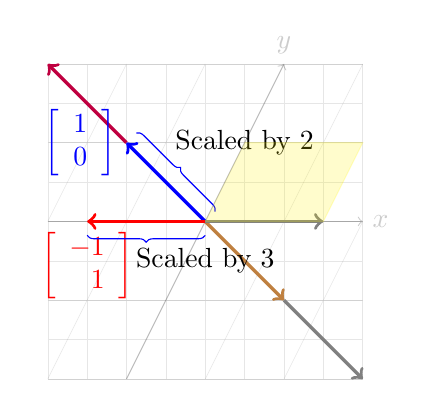
\begin{tikzpicture}[scale=0.5,domain=-2:2]
			\draw[very thin,color=gray,opacity=0.2] (-4,-4) grid (4,4);
			\draw[very thin,color=gray,opacity=0.2] (-4,0) -- (4,0) ;
			\draw[very thin,color=gray,opacity=0.2] (-4,2) -- (4,2) ;
			\draw[very thin,color=gray,opacity=0.2] (-4,4) -- (4,4) ;
			\draw[very thin,color=gray,opacity=0.2] (-4,-2) -- (4,-2) ;
			\draw[very thin,color=gray,opacity=0.2] (-4,-4) -- (4,-4) ;

			\draw[very thin,color=gray,opacity=0.2] (-4,-0) -- (-2,4) ;
			\draw[very thin,color=gray,opacity=0.2] (-4,-4) -- (0,4) ;
			\draw[very thin,color=gray,opacity=0.2] (-2,-4) -- (2,4) ;
			\draw[very thin,color=gray,opacity=0.2] (0,-4) -- (4,4) ;
			\draw[very thin,color=gray,opacity=0.2] (2,-4) -- (4,0) ;

			\draw[->,opacity=0.2] (-4,0) -- (4,0) node[right] {$x$};
			\draw[->,opacity=0.2] (-2,-4) -- (2,4) node[above] {$y$};

			\draw[very thick,->,color=brown] (0,0)--(2,-2) node[left]{};
			\draw[very thick,->,color=purple] (-2,2)--(-4,4) node[left]{};
			\draw[very thick,->,color=gray] (2,-2)--(4,-4) node[left]{};

			\draw[very thick,->,color=blue] (0,0)--(-2,2) node[left]{$\left[\begin{array}{r}
							1 \\
							0 \\
						\end{array}\right]$};
			\draw[decorate,decoration={brace,mirror,raise=5pt},blue] (0,0)--(-2,2);
			\node at (1,2) {Scaled by 2};

			\draw[very thick,->,color=gray] (0,0)--(3,0) node[below]{};
			\draw[very thick,->,color=red] (0,0)--(-3,0) node[below]{$\left[\begin{array}{r}
							-1 \\
							1  \\
						\end{array}\right]$};
			\draw[decorate,decoration={brace,raise=5pt},blue] (0,0)--(-3,0);
			\node at (0,-1) {Scaled by 3};

			\filldraw[color=yellow,opacity=0.2] (0,0) -- (3,0) -- (4,2) -- (1,2);
		\end{tikzpicture}

		\hfill
		$$A = \left[\begin{array}{rr}
					3 & 1 \\
					0 & 2 \\
				\end{array}\right]$$\\[0.2cm]
		The vector representing the line is called the eigenvector of the matrix A.\\[0.2cm]
		特征向量:$\left[\begin{array}{r}
					1 \\
					0 \\
				\end{array}\right],\left[\begin{array}{r}
					-1 \\
					1  \\
				\end{array}\right]$\\[0.2cm]
		The eigenvalue of the matrix A is just the factor by which it stretched or squashed during the transformation.\\[0.2cm]
		特征值:$2,3$
	\end{multicols}
\end{frame}

\begin{frame}{Eigenvalue \& Eigenvector}
	So maybe you can tell why we can get eigenvalue of matrix from this equation:
	$$Ax = \lambda x$$
\end{frame}


\section{参考文献示例 Refference}
\begin{frame}{Refference}
	\begin{multicols}{2}
		\begin{itemize}
			\item Introduction to Linear Algebra(Strang)
			\item Essense of Linear Algebra @3Blue1Brown
			\item Linear algebra and its applications 4th
		\end{itemize}
		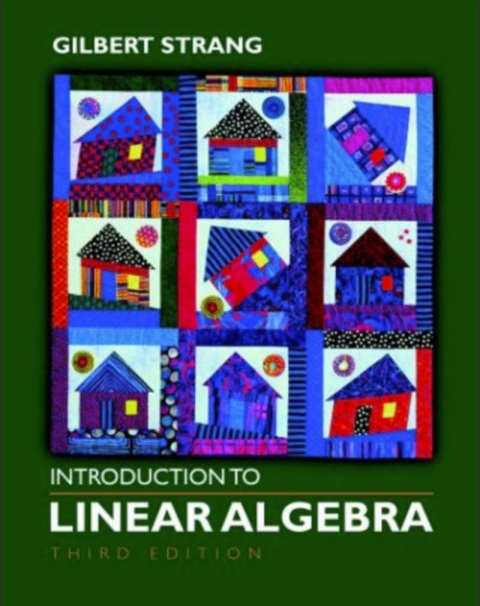
\includegraphics[scale=0.3]{fig/ref1.png}
	\end{multicols}
\end{frame}



\begin{frame}{Acknowledgements}
	\begin{center}
		\begin{minipage}{1\textwidth}
			\setbeamercolor{mybox}{fg=white, bg=black!50!blue}
			\begin{beamercolorbox}[wd=0.70\textwidth, rounded=true, shadow=true]{mybox}
				\LARGE \centering Thank you for listening!  %结束语
			\end{beamercolorbox}
		\end{minipage}
	\end{center}
\end{frame}

% -----------------------------------------------------------------------------
\end{document}